\documentclass[conference]{IEEEtran}
\usepackage{microtype,mathtools,amsmath,multibib,amsfonts,multicol,array,multirow,place ins,cite,balance,makecell,algorithm,algorithmic,subfigure,paralist}
%\usepackage{flushend}
\usepackage{graphicx}
\usepackage{listings}
\usepackage{url}
\usepackage[font=small,labelfont=bf]{caption}

\usepackage{xspace}
\usepackage{color}
\usepackage{ifthen}
\usepackage{fancybox}


\graphicspath{{zu/}}
\DeclareGraphicsExtensions{.pdf,.jpeg,.png}
\hyphenation{op-tical net-works semi-conduc-tor}


\begin{document}
\title{Title}

\author{
\IEEEauthorblockN{Thai Pangsakulyanont\IEEEauthorrefmark{1}, Patanamon Thongtanunam\IEEEauthorrefmark{2},  Daniel Port\IEEEauthorrefmark{3}, Hajimu Iida\IEEEauthorrefmark{2}}
\\
\IEEEauthorblockA{
\IEEEauthorrefmark{1} Kasetsart University, Thailand\\
b5410545036@ku.ac.th
}

\IEEEauthorblockA{
\IEEEauthorrefmark{2} Nara Institute of Science and Technology, Japan\\
patanamon-t@is.naist.jp, iida@itc.naist.jp\\
}

\IEEEauthorblockA{
\IEEEauthorrefmark{3} University of Hawaii at Manoa, USA\\
dport@hawaii.edu \\
}
}


\maketitle
\newboolean{showcomments}
\setboolean{showcomments}{true} % toggle to show or hide comments
\ifthenelse{\boolean{showcomments}}
{\newcommand{\nbnote}[2]{
  % \fbox{\bfseries\sffamily\scriptsize#1}
  \fcolorbox{blue}{yellow}{\bfseries\sffamily\scriptsize#1}
  {\sf\small\textit{#2}}
  % \marginpar{\fbox{\bfseries\sffamily#1}}
 }
}
{\newcommand{\nbnote}[2]{}
 \newcommand{\version}{}
}
\newcommand\pick[1]{\nbnote{Pick sez}{\textcolor{magenta}{#1}}}
\newcommand\thai[1]{\nbnote{Thai sez}{\textcolor{blue}{#1}}}
\newcommand\TODO[1]{\textcolor{red}{\textbf{TODO} #1}}


\begin{abstract}
Software code review is an established method regarded as a best practice in Software Engineering to achieve a sufficient quality in software project. This method mainly intend to early identify defect before integrating changes. Nowadays, Modern Code Review (MCR)\cite{Bacchelli2013a}, less formal and lightweight code reviews have received much attention and  put into software development regularly in both industrial and OSS projects. A main benefit of MCR is the in-person meeting is not required as the formal inspection \cite{Fagan:1976:DCI:1661010.1661012}. Reviewers can discuss to find defects by comments through code review tool or mailing list. Then, developers will fix their changes following those comments. 
% the freeform style of modern code review

% some comments are not technically contributing


\begin{IEEEkeywords}
Modern Code Review, Software Quality, Text Mining
\end{IEEEkeywords}
\end{abstract}

\section{Introduction}
Software code review is an established method regarded as a best practice in Software Engineering to achieve a sufficient quality in software project. This method mainly intend to early identify defect before integrating changes. Nowadays, Modern Code Review (MCR)\cite{Bacchelli2013a}, less formal and lightweight code reviews have received much attention and  put into software development regularly in both industrial and OSS projects. A main benefit of MCR is the in-person meeting is not required as the formal inspection \cite{Fagan:1976:DCI:1661010.1661012}. Reviewers can discuss to find defects by comments through code review tool or mailing list. Then, developers will fix their changes following those comments.

As the performance of code review straight forward to the quality of software project, many studies investigated the influencing factors in MCR\cite{Baysal2001,Mcintosh,Beller,Hamasaki2013}. However, very little research investigate that in MCR, how does a discussion for a proposed change impact to the software quality. Since most of the proposed change improvements are triggered from reviewer comments \cite{Beller}. 
It is possible that comments of reviewers can be either positively contribute the proposed changes or a discussion which is out of scope.
To determine the impact of discussion in MCR, a manual classification is required as study of Beller et. al. \cite{Beller}. As a massive amount of changes and comments in MCR history\cite{Balachandran2013,Thongtanunam2014}, it is painstaking and time consuming to classify data sets to perform quantitative analysis. Moreover, the comments in MCR is unstructured natural text unlike a checklist in the formal inspection. 
%\pick{Need some connection. Says that Massive amount of commits and comment it would be expensive to manually identify. It's natural language }
\begin{figure}[!t]
\centering
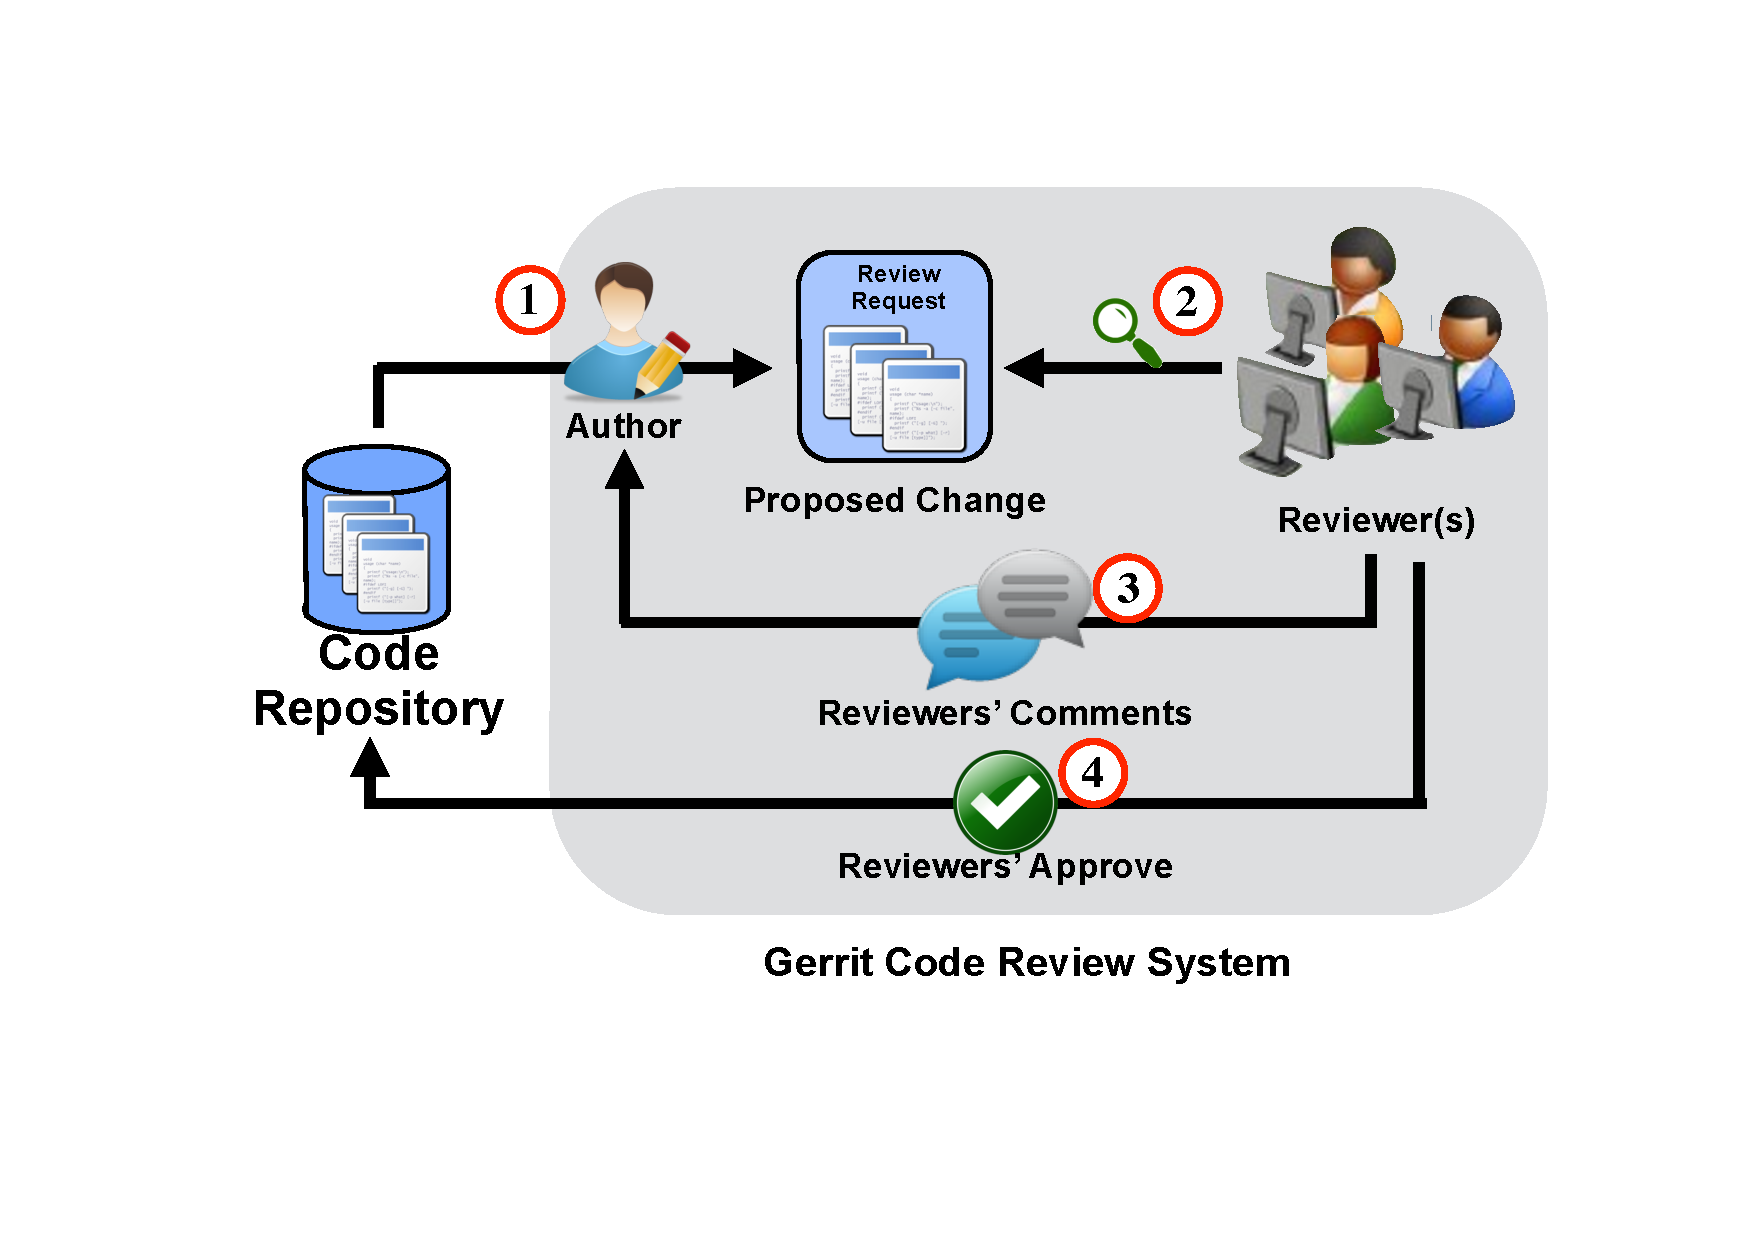
\includegraphics[scale=0.35, trim= 100 110 50 80, clip=true]{review_process}
\caption{An simplified version of MCR Process based on Gerrit system}
\label{fig:process}
\end{figure}

In this paper, we present an approach to automatically classify the usefulness of comments. We define that the usefulness is a comment that contribute to improve the proposed changes. In our approach, we analyze the similarity between commit message of the proposed changes and their comments. Our key idea is that useful comments are likely to contain similar topic as the proposed changes. To do so, we use text mining techniques, Vector Space Model (VSM) to calculate similarity and use euclidian distance to calculate dissimilarity. 
We create our predictive model by estimating a set of similarity and dissimilarity values that best discriminate between a useful and useless comments using the prediction evaluations: Precision, Recall and F-measure.

For our case study, we used a review history of Gerrit\footnote{https://code.google.com/p/gerrit/} system which is tool for supporting MCR process. Our case studied project is Qt\footnote{http://qt-project.org/}, a open source project of a cross-platform application and UI framework supported by Digia corporation. To validate our approach, we manually classify the usefulness for 320 comments and measure its accuracy. We also used our predictive model for the all set of comments to preliminary estimate quality of reviews. According to this, we address the following two research questions:

\noindent \textbf{RQ1:} Can we identify useful and useless discussions in code review?\\
\noindent \textbf{RQ2:} Do code reviewers intensively discuss on the proposed changes?\\
\noindent \textbf{RQ3:} Is this a cost-efficient way to identify useful and useless comments?

\noindent The main contribution of this paper are:
\begin{itemize}
\item We propose an approach to mine natural text of comments in code reviews and classify their usefulness.
\item The experimental results show that our approach can classify comments with XX of F-measure.
\item We found that XX\% of comments for each review are classified as useful comments, while XX \% of comments are classified as useless comments.
\end{itemize} 
%Software Inspection is basically composed of a three-step procedure: preparation, inspection meeting, and repair.

%Motivation Example.\thai{Wow}


%\section{Background}
%In this section, we describe MCR process based on Gerrit system. Then, we describe the background behind our approach composed of text mining techniques using VSM and euclidian distance and prediction evaluation techniques. 
\section{Modern Code Review Process}

An overview of MCR process based on Gerrit system is shown in Figure \ref{fig:process}. The grey area shows the review process of the system which composed of four main steps. (1) an author creating a patch and submitting a set of new or modified files as a review request to Gerrit system. (2) reviewers examine the proposed code changes whether it contains defects or not. (3) reviewers will give comments where should the author improve the code change. The author will create a new change according to the comments then re-submit a new patch again. Then, reviewers will examine the new change. If there is still a needed improvement, reviewers will give comments to fix again. The steps (1)-(3) will be iterated until reviewers can determine that this changes can be merge to the project or should not be merge (reject the change). 

According to this process, reviewers' comment is the most important for the software quality. McIntosh et. al. \cite{Mcintosh} also found that components which were reviewed without discussion are likely to contain bugs. However, as tool supporting MCR allows reviewers freely write a message to the author, it is often seen that some comments are not clearly identify defects and ineffective. Microsoft developers reported that they only focus on minor logic errors rather than discussing deeper in design\cite{Bacchelli2013a}. Our observation in Qt project also correspond this finding. We found some comments are superficial and unrelated to the proposed changes. For example, a superficial and unconfident reviewer as shown in Fig. \ref{fig:example}(a), a comment for rule of using Version Control System (e.g. Git) in the project Fig. \ref{fig:example}(b). 

\begin{figure}[!t]
\centering
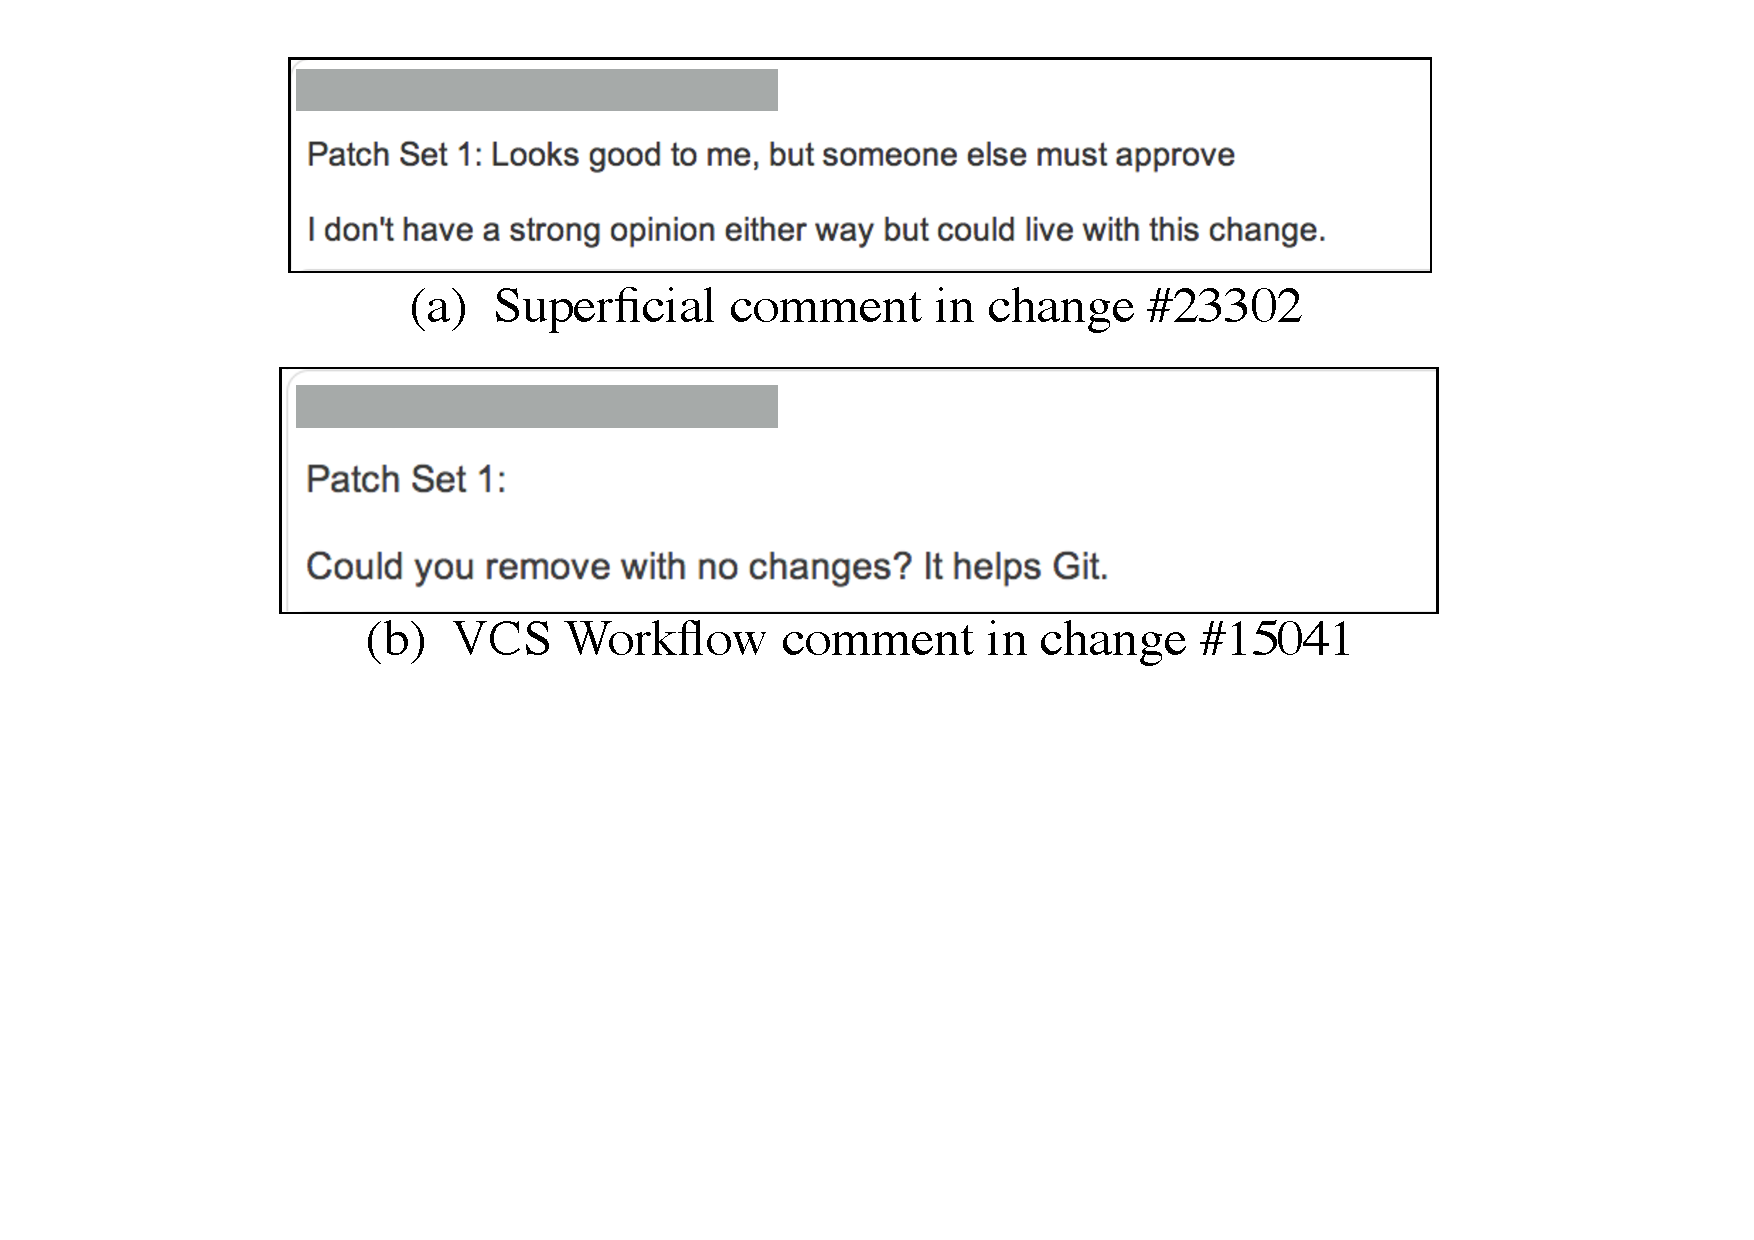
\includegraphics[scale=0.4, trim= 100 250 0 0, clip=true]{comment_examples}
\caption{Examples of comment in code reviews of Qt project.}
\label{fig:example}
\end{figure}




\section{Reviewers' Comments Classification Approach}
\begin{figure}[!t]
\centering
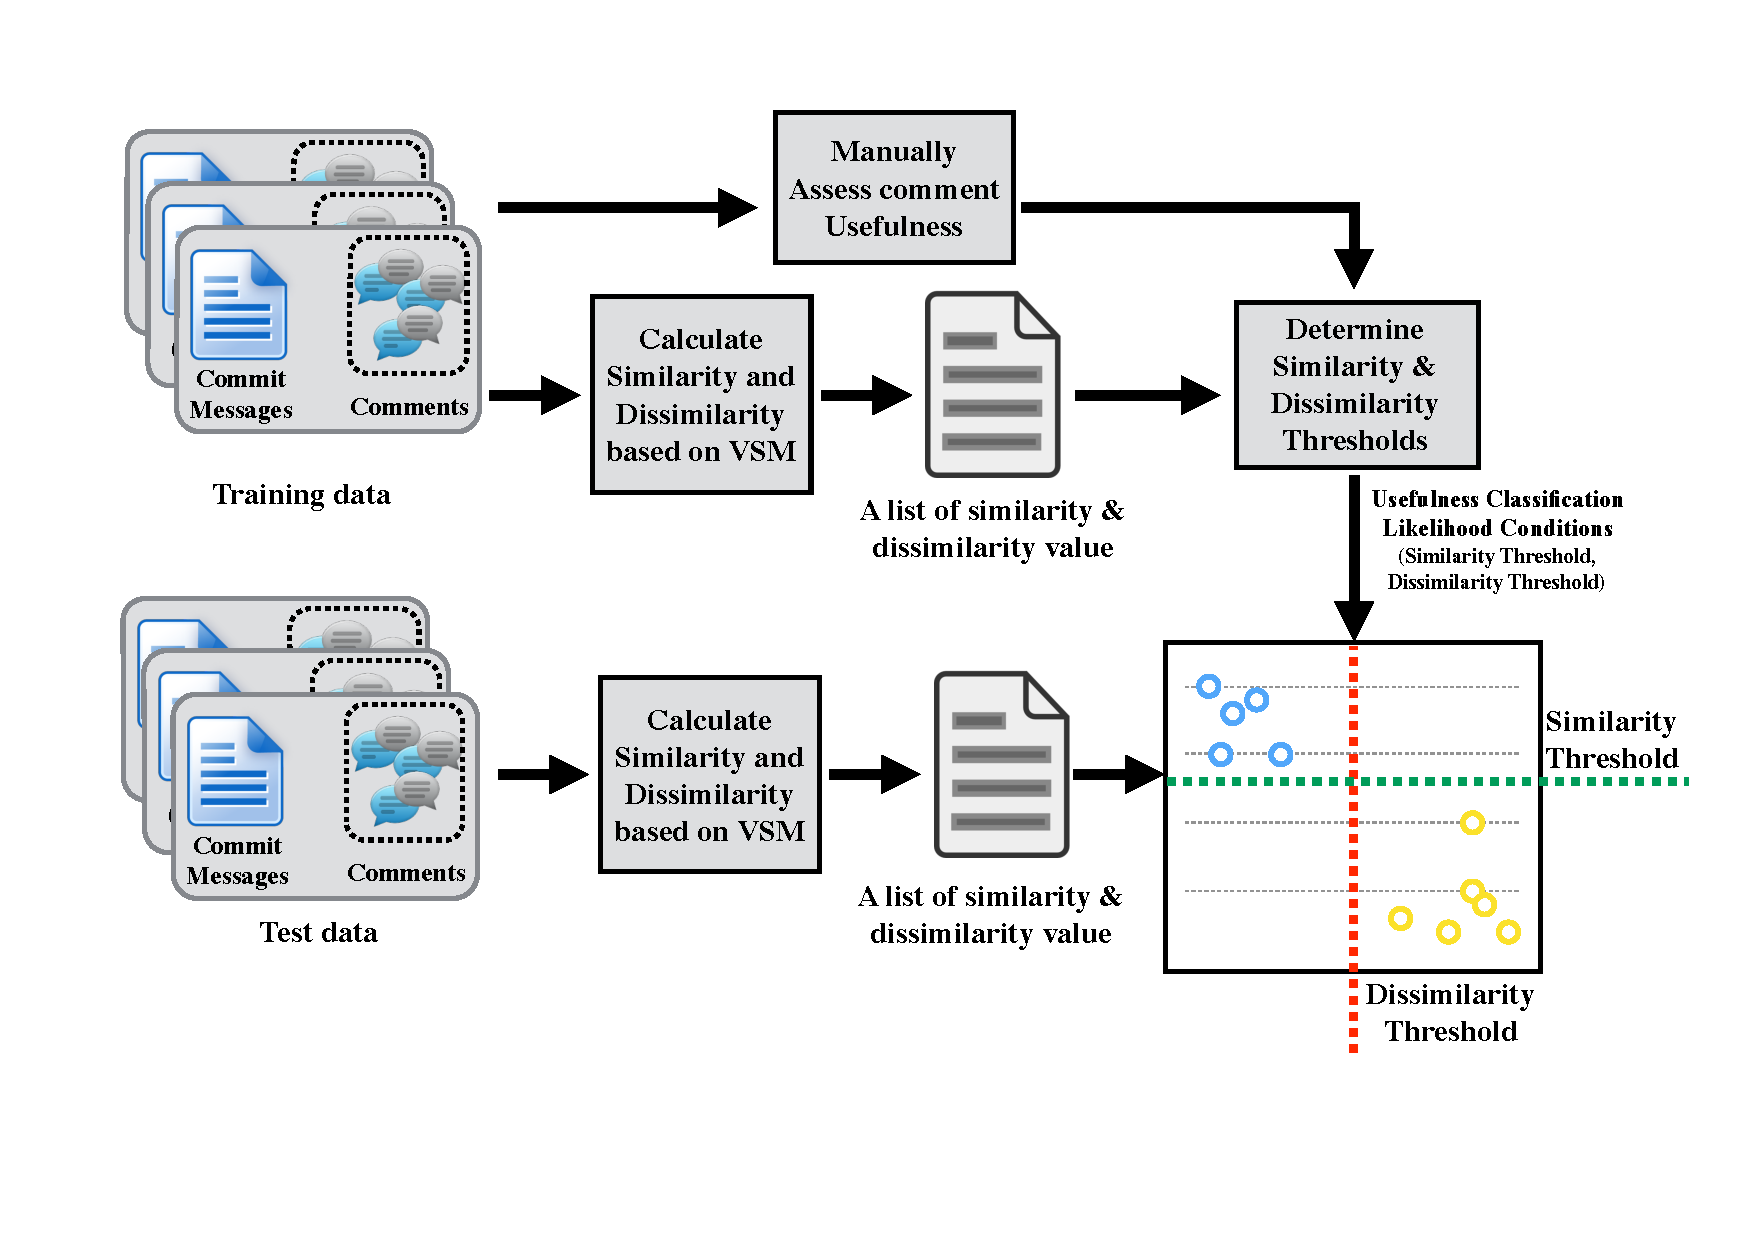
\includegraphics[scale=0.35, trim = 50 90 0 30, clip=true]{overview2}
\caption{Overview of our classification approach.}
\label{fig:overview}
\end{figure}

Figure \ref{fig:overview} shows the overview of our proposed approach. We classify usefulness of comments by measuring similarity between commit message of proposed change and its comments. To calculate similarity in Fig. \ref{fig:overview}(a), we use Vector Space Model (VSM) which is well-known technique for retrieving similar documents written in unstructured natural language. We also use euclidian distance to calculate dissimilarity. For our training dataset, we manually identify every pair of comment and commit messages in Fig. \ref{fig:overview}(b). Then, we use the results from Fig. \ref{fig:overview}(a) and from Fig. \ref{fig:overview}(b) to estimate similarity and dissimilarity threshold that can best discriminate useful/useless comments. Using these thresholds, we can classify the usefulness of comments for the rest of comments in review history. 

To classify usefulness of comment using similarity and dissimilarity, we firstly formalize our classification model as follows:
\begin{itemize}
\item $\Theta(c,S_T,D_T)$ predict as \textbf{useful} if $\mathrm{sim}(m,c) \geq S_T$ and $\mathrm{dist}(m,c) \leq D_T$.
\item $\Omega(c,S'_T,D'_T)$ predict as \textbf{useles} if $\mathrm{sim}(m,c) \leq  S'_T$ and $\mathrm{dist}(m,c) \geq D'_T$.
\end{itemize}
where $S_T$ and $D_T$ are similarity and dissimilarity thresholds for useful comments identification; while $S'_T$ and $D'_T$ are similarity and dissimilarity thresholds for useless comments identification. The functions $\mathrm{sim}(m,c)$ and $\mathrm{dist}(m,c)$ calculates similarity and dissimilarity of comment $c$ comparing with commit message of its review. The details our approach is described in the following subsections.
\pick{Why we need two measurements?}
\pick{What happen in model for otherwise?}

\subsection{Similarity and Dissimilarity Calculation based on VSM}
%Vector Space Model (VSM) is well-known technique for information retrieval where documents written in unstructured natural language. In Software Engineering, VSM has been widely use to find relationship among documents in software issue tracking system\cite{Davies2012}.
For each review, we compute similarity and dissimilarity of every comments comparing with the commit message which is described the purpose of the change.
To do so, we use VSM which is a model for representing text documents as vectors. For a set of commit messages and comments ($D$), each document, $d$ (commit message or comment) is represented as $\overrightarrow{V_d} = <w_{1,d},w_{2,d},w_{3,d},...w_{n,d}>$, where $n$ is the total number of unique terms occur in $D$. The $w_{t,d}$ value is TF-IDF weighting of term $t$ calculated from term occurrence frequency using Equation \ref{eq:tf-idf} where $tf_{t,d}$ is frequency of term $t$ occurs in document $d$; and $|\{d' \in D | t \in d'\}|$ is the number of other documents $d'$ that also contain term $t$.  

\begin{equation}
w_{t,d} = tf_{t,d} \times \log\frac{|D|}{1+|\{d' \in D | t \in d'\}|}
\label{eq:tf-idf}
\end{equation}

After transforming commit message and comments to vectors, we calculate similarity using Cosine similarity and Euclidian distance. 


\noindent\textbf{Cosine similarity} measures similarity between two vectors using inner product. Given a vector commit message $\overrightarrow{V_m}$ and the vector of its comments $\overrightarrow{V_m}$, we can calculate Cosine similarity using Equation \ref{eq:cosine}. The similarity value is ranging $[0,1]$ where 0 means there is no similarity and 1 means two vectors are textually similar.  

\begin{equation}
\mathrm{sim}(m,c) = \cos\theta(\overrightarrow{V_m},\overrightarrow{V_c}) = \frac{\sum_{i=1}^{|D|} w_{i,m} \times w_{i,c}}{\sqrt{\sum_{i=1}^{|D|} w^2_{i,m} \times \sum_{i=1}^{|D|} w^2_{i,c}}}
\label{eq:cosine}
\end{equation}

\noindent\textbf{Euclidian distance} measures ordinary distance between each element of two vectors using Equation \ref{eq:euclid}. We can use this distance as an dissimilarity. Given a vector commit message $\overrightarrow{V_m}$ and the vector of its comments $\overrightarrow{V_m}$, we can calculate Euclidian distance using Equation \ref{eq:cosine}. The distance value is ranging $[0,\infty)$ where 0 means these vectors are the same vectors while a more distance means these vectors are less similar.

\begin{equation}
\mathrm{dist}(m,c) = \mathrm{euclidian}(\overrightarrow{V_m},\overrightarrow{V_c}) = \sqrt{\sum_{i=1}^{|D|}(w_{i,m} - w_{i,c})^2}
\label{eq:euclid}
\end{equation}

\subsection{Estimating Similarity and Dissimilarity Threshold}
We find similarity and dissimilarity thresholds by selecting $s_t,d_t$ values that can maximize $\mathrm{F\text{-}measure}_{s_t,d_t}$. This is an accuracy measurement for a binary classification considering an accuracy of prediction (precision) and  a coverage of classification (recall). This can be calculated using Equation \ref{eq:fmeasure}.

\begin{equation}
\begin{split}
\mathrm{F\text{-}measure}_{s_t,d_t} &= 2 \times \frac{\mathrm{precision}_{s_t,d_t} \times \mathrm{recall}_{s_t,d_t}}{\mathrm{precision}_{s_t,d_t} + \mathrm{recall}_{s_t,d_t}}
\\
\mathrm{precision}_{s_t,d_t}  &= \frac{\mathrm{TP}_{s_t,d_t}}{\mathrm{TP}_{s_t,d_t}+\mathrm{FP}_{s_t,d_t}}
\\
\mathrm{recall}_{s_t,d_t}  &= \frac{\mathrm{TP}_{s_t,d_t}}{\mathrm{TP}_{s_t,d_t}+\mathrm{FN}_{s_t,d_t}}
\end{split}
\label{eq:fmeasure}
\end{equation}




Suppose we use $\Theta(c,S_T=s_t,D_T=d_t)$ as predict model to identify useful comments , $\mathrm{TP}_{s_t,d_t}$ is the number of comments that our model predicted as \textit{useful} and are actually useful; $\mathrm{FP}_{s_t,d_t}$ is the number of comments that our model predicted as \textit{useful} but are actually useless; and $\mathrm{FN}_{\theta_s,\theta_d}$ is the number of comments that our model predict as \textit{useless} but are actually useful. To measuring F-measure for $\Omega(c,S_T=s_t,D_T=d_t)$ model, it uses the same consideration but change the determination to useless comments. For the correctness of prediction, we determine from the useful/useless defined dataset. 


%Using this method, we iteratively measure an accuracy for values of $s_t$ and $s'_t$ ranging $[0,1]$; and values of $d_t$ and $d'_t$ ranging $[0,\infty)$. 

%\begin{equation}
%\mathrm{F\text{-}measure}_{S_T,D_T} = \frac{2\mathrm{TP}_{S_T,D_T}}{2\mathrm{TP}_{S_T,D_T}+\mathrm{FP}_{S_T,D_T}+\mathrm{FN}_{S_T,D_T}}
%\label{eq:precision}
%\end{equation}

%where $\mathrm{TP}_{S_T,D_T}= |\{ c \in C |  \text{\textbf{useful}}(c,S_T,D_T) = \mathrm{TRUE} \}\cap \{c \in C| \mathrm{vote}(c) = 2\}|$,  $\mathrm{FP}_{S_T,D_T} = |\{ c \in C | \text{\textbf{useful}}(c,S_T,D_T) = \mathrm{FALSE} \}\cap \{\mathrm{vote}(c) = 2\} $, $\mathrm{FN}_{S_T,D_T} = |\{ c | c \in C, \text{\textbf{useful}}(c,S_T,D_T) = \mathrm{TRUE} \}\cap \{\mathrm{vote}(c) < 2\} $
%According to this, we can formalize as follows:

%\begin{equation}
%(S_T,D_T) = \max(\{\mathrm{F\text{-}measure} \text{ of \textbf{useful}}(c,s_T,d_T) | s_T\in[0,1] \text{ and } d_T\in [0,\infty) \})
%\end{equation}






\section{Case Study Design}


We used the review history of Qt project from Gerrit code review tool provided by Hamasaki et. al. \cite{Hamasaki2013}. Qt project is a large open source project composed of small subsystems. For our case study, we selected the most active subproject \texttt{qtbase} project. From this project, we used the review history from \TODO{Month-Year} to \TODO{Month-Year} which has \TODO{XX} reviews and \TODO{XX} comments.


% where we got the data
%We used the review data sets of the Qt project collected by Hamasaki et al\cite{Hamasaki2013}.
%Only reviews in the master branch of \texttt{qtbase} project are considered,
%as it is the most active branch.

% quick structure
%\pick{This already explain in background :D}
%Each change includes a \emph{commit message} which describes what is changed.
%After a change is submitted to Gerrit, reviewers can give scores to it.
%The scores will determine whether the change will be accepted or not.
%Reviewers can also add comments to the change, which may optionally be added to a specific line of code inside a changed file.
%Majority of the comments are automatically generated by Gerrit and do not contain any user-written text.

% overview
%In our classification method,
%all commit messages and comments that are human-written are converted into vectors using tf--idf algorithm.
%Few comments are sampled and then classified manually for use in training and validation.
%A model is created from these training data, from which useful comments can automatically be identified.
%This process is illustrated in Fig.\ref{fig:overview}.
%



\subsection{Data Preparation}
We used commit messages and comments in the dataset. Before classifying the usefulness of comments, we firstly processed the commit message and comments as follows: 

\subsubsection{Automatically generated messages removal}
In Gerrit, the comments are composed of comment messages from reviewers and automated messages. These automatic messages are generated by Gerrit and integration system to record activities, for example, \textit{'Upload patch set 1.'}, \textit{'Change has been successfully cherry-picked to the staging branch as ...'}. Since these messages are not impact to software quality\cite{Mcintosh}, we removed them from our data set. We identified these automatic messages using regular expression and selecting frequently appeared pattern of messages.  


%The commit messages and all comment texts are converted into vectors as part of the preparation step.
%Fig. \ref{fig:preprocess} illustrates the overview of this step.
%We wrote scripts in Ruby language to perform these tasks.

%\begin{figure}[h]
%\centering
%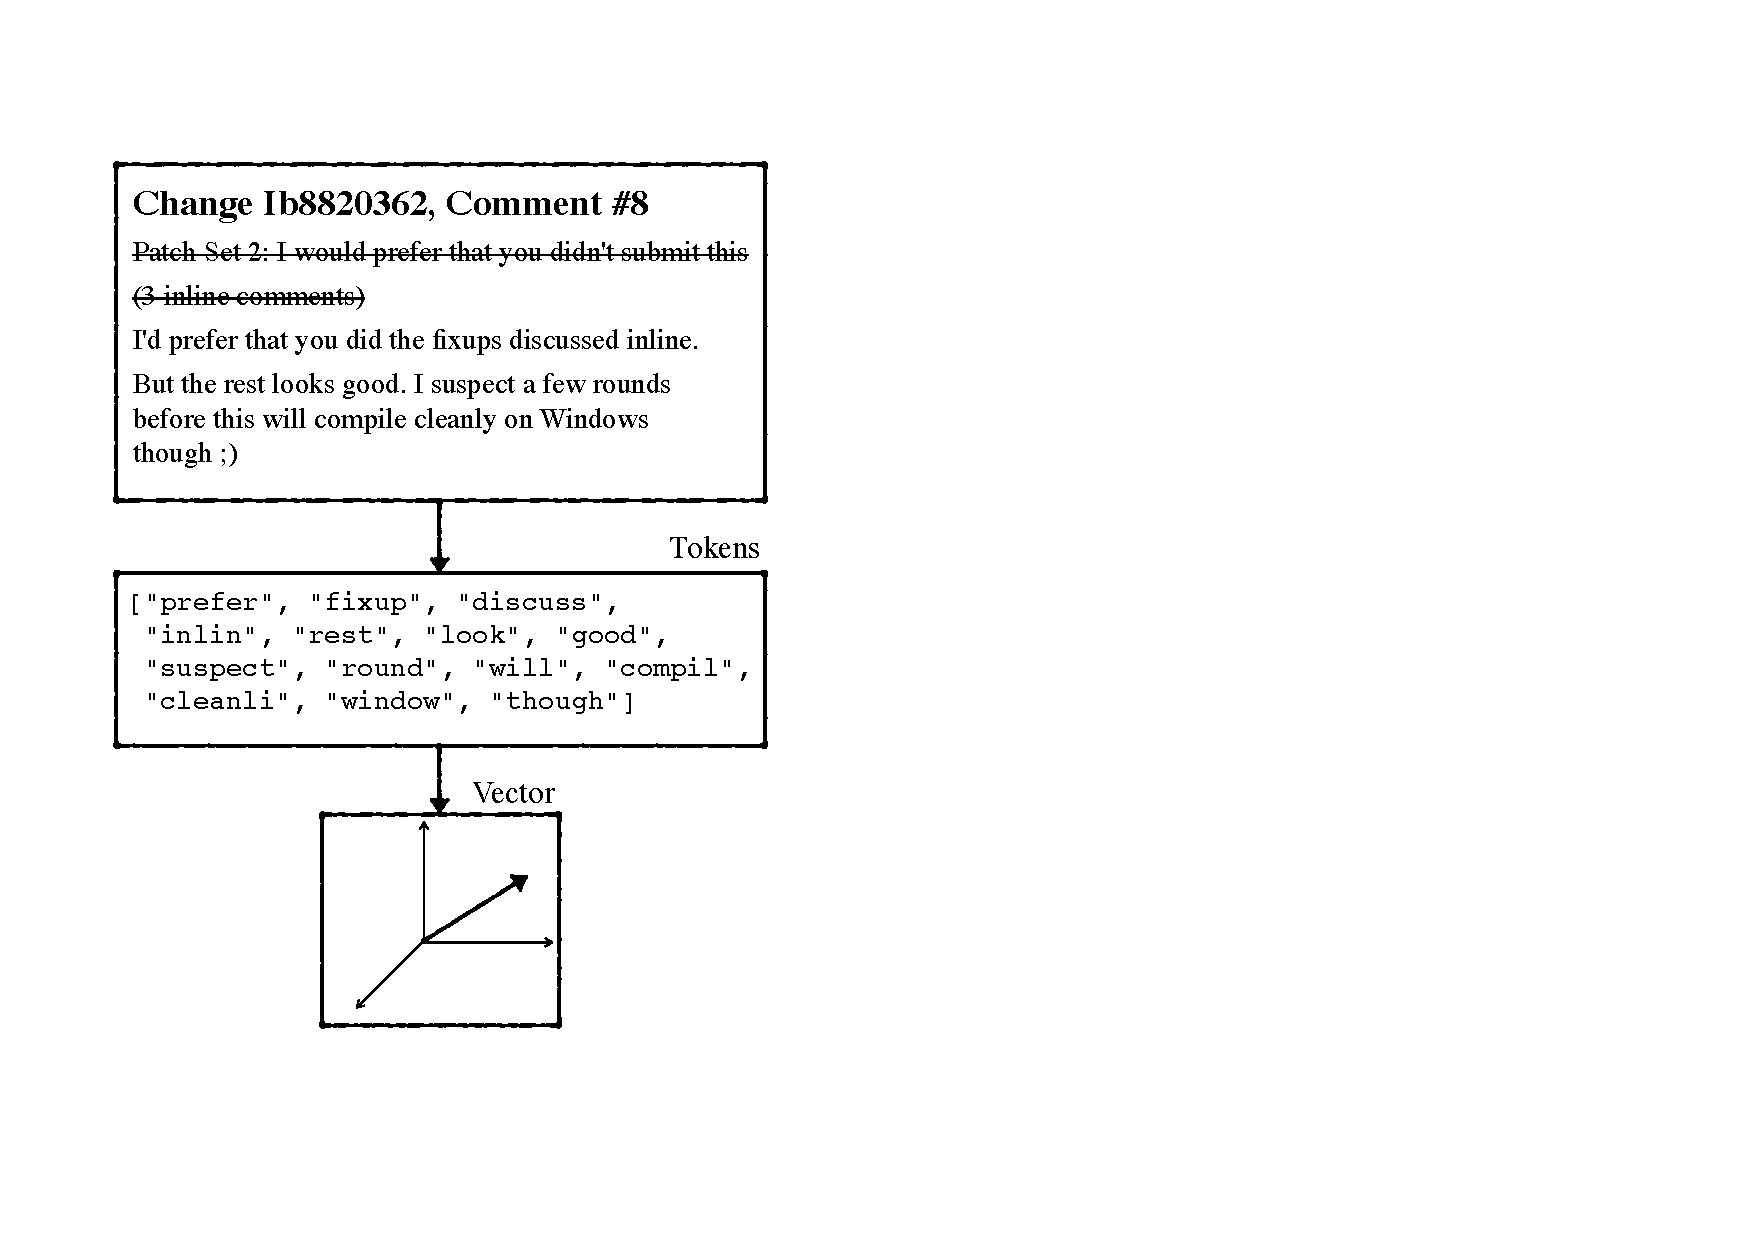
\includegraphics[width=3in]{preprocess}
%\caption{The data preparation process.
%Automatically generated texts are removed, remaining text is tokenized, stop words are removed, remaining tokens are stemmed,
%and are converted into a vector.}
%\label{fig:preprocess}
%\end{figure}



%\subsubsection{Removal of automatically generated text}
%
%First, all comments by the Gerrit system, \emph{Qt Sanity Bot}, and \emph{Qt Continuous Integration System} are skipped.
%
%% conversion into vector, wow
%Next, we looked for common patterns that appeared in the comments, because it is very likely that they are automatically generated.
%This is accomplished by splitting texts into lines, and for each line, searching for words that can be found in the English wordlist\footnote{The wordlist found in \texttt{/usr/share/dict/words} from Ubuntu Linux distribution is used.}.
%This effectively removed the ID numbers and other non-generic terms.
%
%Next, the lines that appears most frequently are identified.
%From these lines, we then constructed the regular expression patterns,
%and finally, these patterns are used to filter out automatically generated text from our data.



\subsubsection{Data Preprocessing}
 we extracted semantic words commit messages and comment messages before converting to vector. For each message, we removed all punctuation signs, digits, and common words (e.g. a, an, the) using Google stop word list\footnote{Available at \url{http://meta.wikimedia.org/wiki/Stop_word_list/google_stop_word_list#English}}. We then used Porter stemming algorithm to remove the commoner morphological and inflexional endings from words in English.
 


%After the automatically generated messages are removed, we extracted the words in each document into a list of tokens by searching for alphanumeric characters including apostrophes.
%Stop words from the Google stop word list\footnote{Available at \url{http://meta.wikimedia.org/wiki/Stop_word_list/google_stop_word_list#English}} are then removed.
%The stemming is performed on remaining tokens using Porter stemming algorithm.
%The remaining words are then combined to form a corpus of all used words.



%\subsubsection{Conversion into vector}
%
%Finally, the tf--idf algorithm is used to convert each document into a vector.

\subsubsection{Ground-Truth Data Preparation}
To prepare ground-truth data, we read comments and manually identified useful and useless comments. In this study, we use three people (the first two authors and one student) independently classify comments by giving a question that ``Does this comment technically contribute to its change or not?''. Then, the readers gave a vote for \texttt{YES} if the comment is likely to useful and \texttt{No} if the comment is likely to useless. From the voting scores, we regarded that the comments with three \texttt{YES} votes are \textbf{useful} comments and the comments with no \texttt{YES} votes (i.e. three \texttt{NO} votes) are \textbf{useless} comments. For the comments with one and two \texttt{YES}' votes, we remained them as \textbf{unclear} comments which we cannot confidently defined. 

\subsection{Research Questions}
To validate our approach, we addressed the following research questions:

\noindent \textbf{RQ1: Can we identify useful and useless discussions in code review?}\\
\indent To answer this question, we randomly sampled 320 comments from our data set and manually identified usefulness as described in previous subsection. Then, we used these comments for both training and test data set for our approach to determine an effectiveness of our approach. We also determined the robustness of our approach using cross validation. We randomly selected 90\% of 320 comments for training set and 10\% for test set.
The effectiveness was measured using precision, recall and F-measure as described in Equation \ref{eq:fmeasure}. We repeated this validation for 300 times and find average of accuracy.

Since our models do not include unclear type of comments, we defined them as negative condition i.e useless comments in case of useful classification (when using $\Theta(c,S_T,D_T)$ model) and useful comments in case of useless classification (when using $\Omega(c,S'_T,D'_T)$ model).


%We sampled 320 comments from the data set.
%These samples are then classified as either useful (that is, technically contributing to the software) or not useful.
%This task is carried out by three people who worked independently.
%
%Each comment is then scored based on the number of positive answers.
%For example, a comment with a score of 3 means that all three people said that it is useful,
%while a comment with a score of 0 means that none of us marked it as useful.


\noindent \textbf{RQ2: Do code reviewers intensively discuss on the proposed changes?}\\
\indent To answer this question, we estimated similarity and dissimilarity thresholds using comments from RQ1 for training set. We then used these thresholds to classify the rest of comments. A statical analysis was performed to understand the impact of useful discussion to software quality.

\noindent \textbf{RQ3: Does this approach practical and cost-effective for large-scale projects?}\\
\indent




%\subsection{Training Data}



%The score of a comment can be defined as:

%\begin{align*}
%Score_i & = \sum_{\text{reviewer } r} Review(r, i). \\
%Review(r, i) & = \begin{cases}
%	1 & \text{if } r \text{ says that the comment } i \text{ is useful,} \\
%	0 & \text{otherwise.}
%\end{cases}
%\end{align*}



%\pick{I re-wrote of these, hope I don't miss something ;)}
%\subsection{Model Generation and Validation}
%
%% the metrics
%For each comment, we computed similarity and dissimilarity metrics
%between the comment text and the corresponding commit message.
%We chose cosine similarity and euclidean distance as the metrics to use in model generation.
%
%\begin{figure}[h]
%\centering
%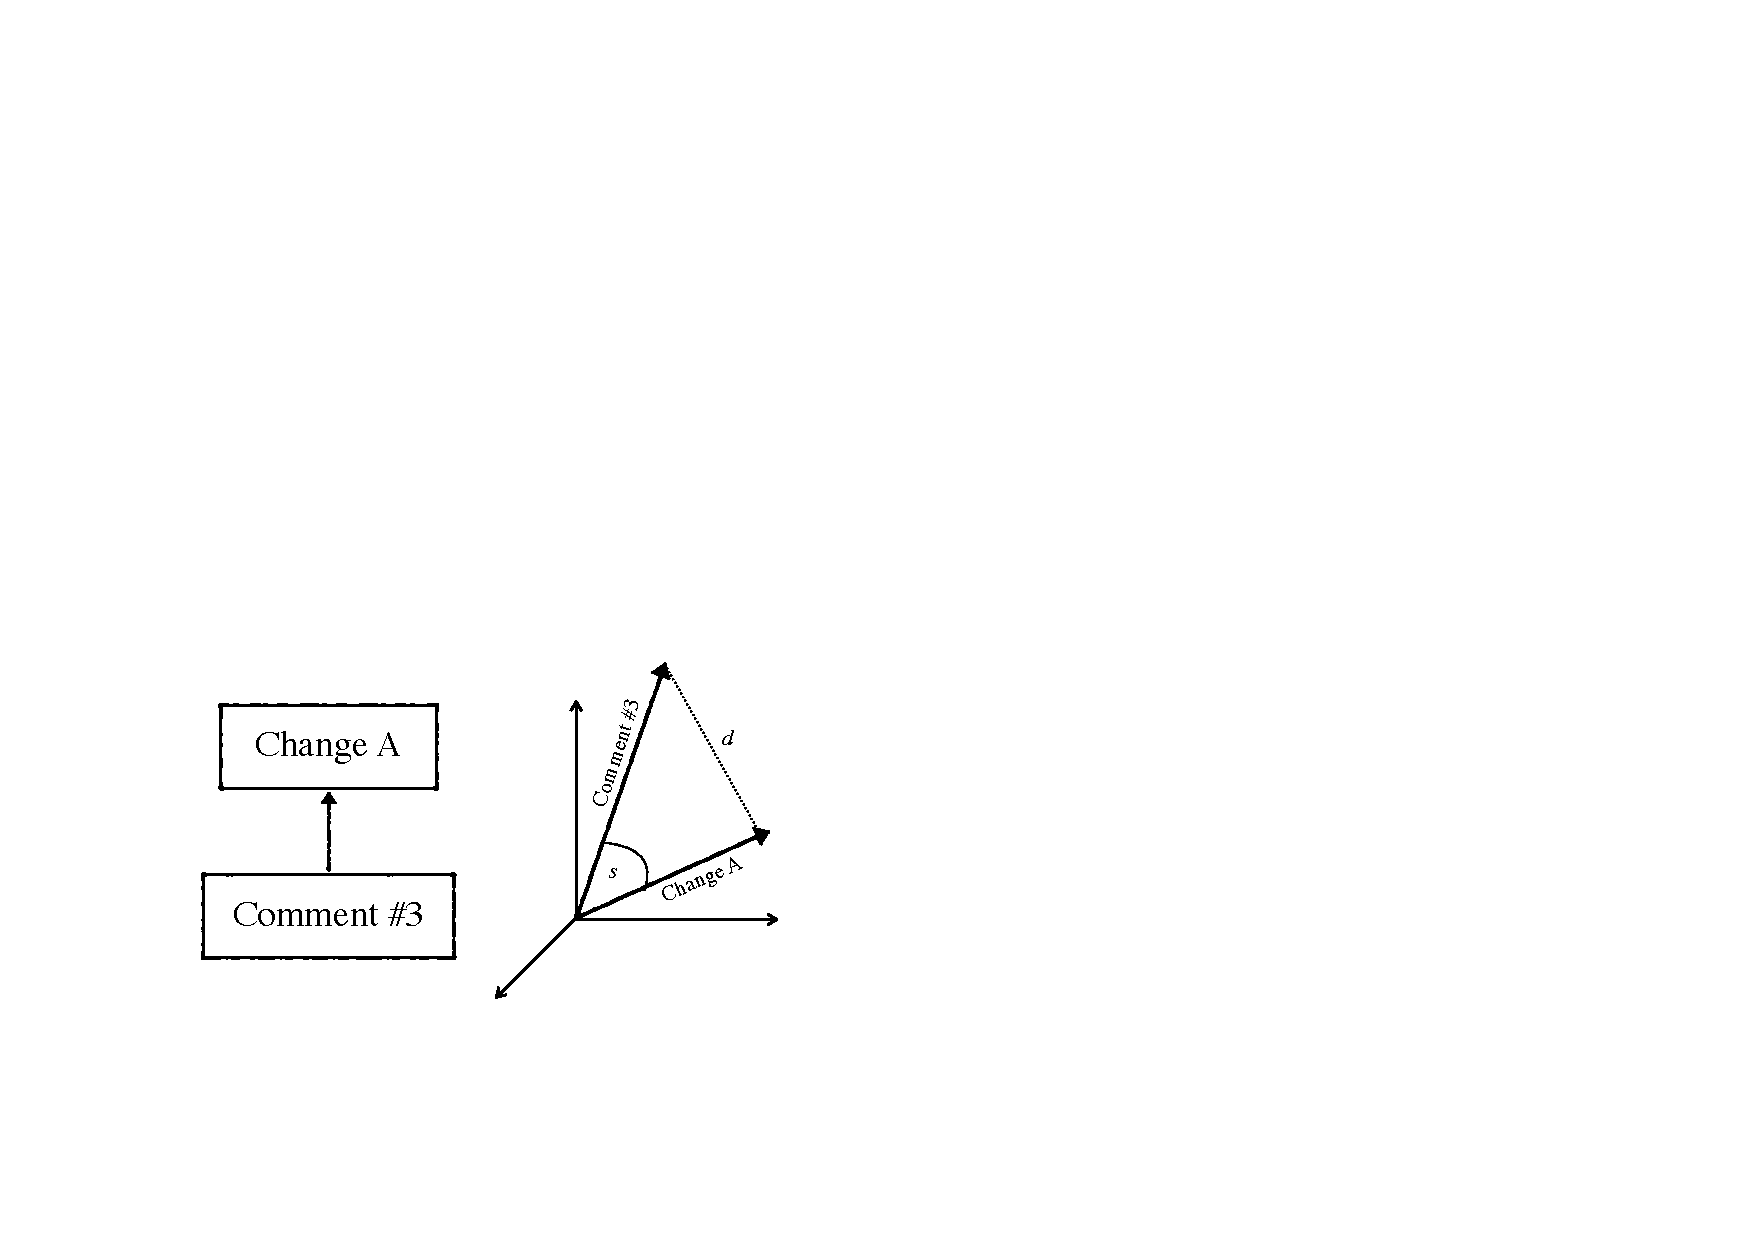
\includegraphics[width=3in]{vector}
%\caption{The similarity and distance metric that is being used.}
%\label{fig:vector}
%\end{figure}
%
%% assumptions in categorization
%The model is based on two assumptions: that useful comments will have a $similarity \geq A \text{ and } distance \leq B$,
%and that comments that are not useful will have a $ similarity \leq C \text{ and } distance \geq D$,
%where $A$, $B$, $C$, and $D$ are some constant.\footnote{We also tried using the `or' operator, and found that using `and' produces better result.}
%
%% finding parameters
%To find these parameters, a brute-force approach is used.
%This is possible because the set of $similarity$ and $distance$ values are discrete.
%Each possible value of $A$, $B$, $C$, and $D$ are evaluated to find the constant that returns the maximum F$_1$ score.
%
%% validation
%To validate our model, we randomly split the data into 10 parts.
%9 parts are used for training, and 1 part for validation.
%This process is repeated 300 times. % while I sleep
%The values of precision, recall, F$_1$ score, and accuracy are recorded and then averaged
%to give the overall performance of our model.


\section{Case Study Results}
\pick{I'm exhausted...sorry. My writing here is pretty bad, hope you understand what I'm trying to say :)}
Table \ref{tb:datastatistic} summarizes data set we used for this study after preparation.
From 72,484 comments of 6,605 reviews with its commit messages extracted from raw data set, there are 10,670 (15\%) of comments are written by reviewers while 85\% of comments are automatically generated by Gerrit system and integration bots.  

\begin{table}[!h]
\caption{A summary data sets and some statistics.}
\centering
\small
\begin{tabular}{ccc}
\hline
& Total Number & Percentage \\ \hline \hline
Commit Messages & 6,605 &  -  \\ \hline
All Comments & 72,484& - \\ \hline
Reviewers Messages & 10,670 & 15\% \\ \hline
Automated Messages. & 61,814 & 85\% \\ \hline 

\end{tabular}
\label{tb:datastatistic}
\end{table}



%\pick{I realize that your figure is better for the presentation :)}
%\begin{figure}[h]
%\centering
%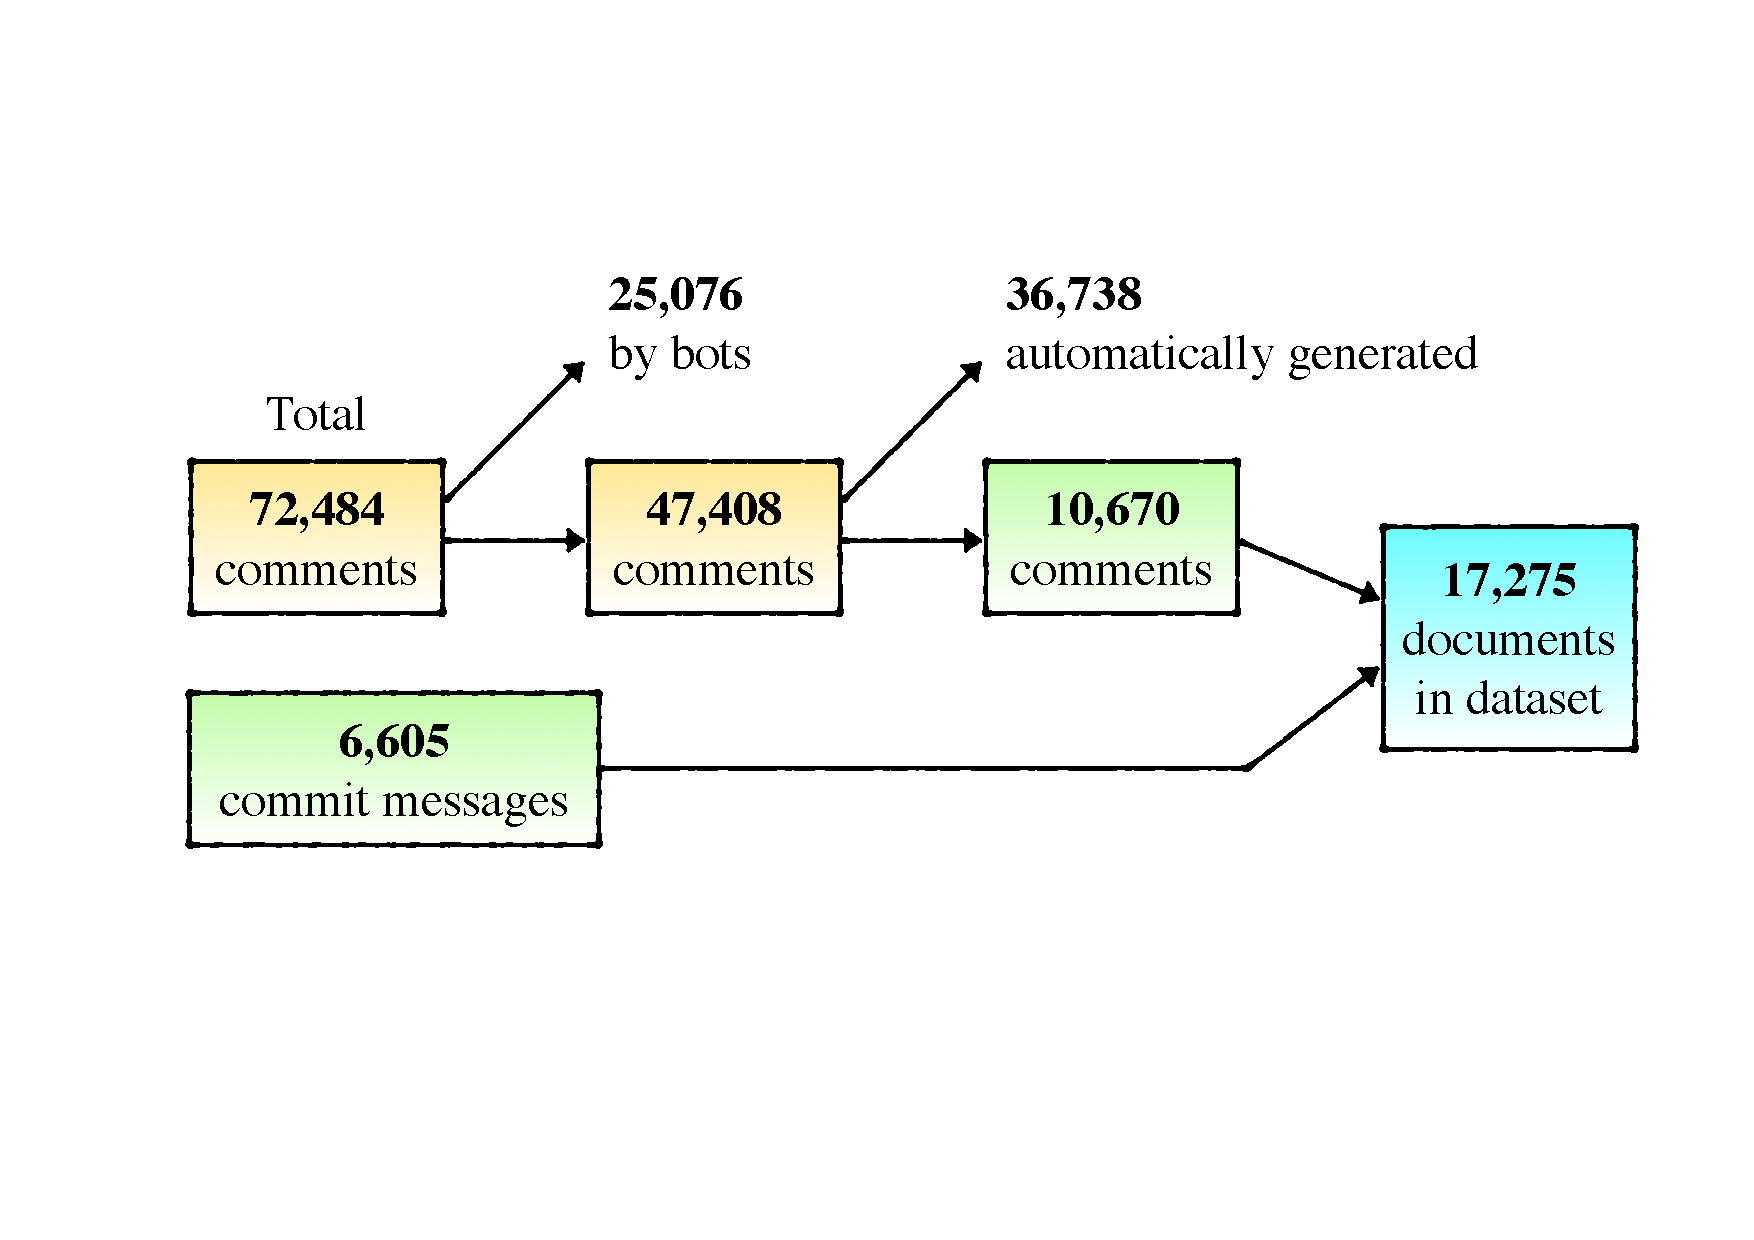
\includegraphics[width=3.2in]{filter}
%\caption{The filtering process.}
%\label{fig:filter}
%\end{figure}
%\subsection{Data Preparation}
%\subsubsection{Data extraction}
%
%6,605 changes and 72,484 comments have been extracted from the raw dataset.
%35\% of the comments are by the system or one of the bots, and are thus discarded.
%
%\subsubsection{Common pattern removal}
%
%By looking for most frequent lines, common patterns were found, such as \emph{`Uploaded patch set 2.'} and \emph{`Change has been successfully cherry-picked to the staging branch as \dots'}.
%
%Removing occurrences of these patterns leaves 77\% of the remaining comments empty.
%This probably means these comments solely contain automatically-generated text, and are thus discarded.
%This leaves us with 10,670 comments and 6,605 commit messages; a total of 17,275 documents.
%
%\subsubsection{Tokenizing}
%
%After the tokenization step, 393,238 tokens are generated in total. They are composed of 20,025 different words.
%This means that each document will be converted into a vector of 20,025 dimensions, each dimension representing a single word.
%


\noindent \textbf{RQ1: Can we identify useful and useless discussions in code review?}

From 320 samples, the number of labeled comments were 87, 60, 51, and 122 for 0, 1, 2, and 3 \texttt{YES} votes, respectively.
To estimated estimated similarity and dissimilarity thresholds, we iterated $s_t$, $d_t$, $s'_t$, and $d'_t$ values from \TODO{.......}. \pick{We cannot brute force for every floating number. How did we calculate this?} Table \ref{tb:thresholds} shows 5 sets of thresholds that best classify useful and useless comments based on F-measure score. \pick{I used dummy results. Please change it} \pick{What we got from this table? What information can we interpret? The threshold is slightly different? Is it good or bad? Please describes.} 

\textbf{Model Effectiveness.} Figure \ref{fig:scatter} shows relationship between comments class and our similarity thresholds. The green area represents useful model $\Theta(c,S_T=0.09028129266684175,D_T= 2.245146382888072)$ and the red area represents useless classification model $\Omega(c,S_T=0.09028129266684175,D_T= 2.245146382888072)$. This figure also shows an example comment that fall in the different area\pick{Didn't put yet}. As shown in the figure, most of comments fall in green area is useful comments and very few useless comments fall in this area. Similarly, most of comments fall in red area is useless comments. However, some comments were not determined (in white area). From the example comment, it shows that these comments discussed on ..... which did not contains any similar words. Moreover, the areas of these two models are overlap. Table \ref{tb:classify_number} summarizes the number of classification from this results. Interestingly, 87\% useless comments classified by our model have \texttt{YES} = 0 and 1 voting scores. This is same as the results of useful class that most of them have \texttt{YES} = 2 and 3 voting scores
This finding suggests that these unclear comments have something.....

\begin{table}[h]
\centering
\small
\caption{Number of comments classified by our approach against ground truth data }
\begin{tabular}{ccccc}
\hline
& \multicolumn{4}{c}{Class from Ground Truth Data} \\ \cline{2-5}
Our&  Useless  & Unclear  & Unclear & Useful \\
Classifications&  (\texttt{YES}=0) & (\texttt{YES}=1) & (\texttt{YES}=2) & (\texttt{YES}=3) \\
\hline \hline
Useless & 69 & 23 & 7 & 6 \\
Useful & 4 & 13 & 24 & 95 \\
Overlap & 1 & 1 & 0 & 1 \\
Undetermined & 12 & 24 & 20 & 20 \\
\hline
\end{tabular}
\label{tb:classify_number}
\end{table}


\begin{table*}[!t]
\caption{An accuracy of similarity and dissimilarity thresholds for useful and useless comment classifications}
\small
\centering
\def\arraystretch{1.2}
\begin{tabular}{ccccccc}
\hline
Prediction Models  & Rank & $s_t$ & $d_t$ & F-measure & Precision & Recall \\ \hline \hline
\multirow{7}{*}{$\Theta(c,S_T=s_t,D_T=d_t)$} & 1 & 0.09028129266684175 & 2.245146382888072 &  1.00000 & 1.00000 & 1.00000 \\ \cline{2-7}
& 2 & 0.09028129266684175 & 2.245146382888072 &  1.00 & 1.00 & 1.00 \\ \cline{2-7}
& 3 & 0.09028129266684175 & 2.245146382888072 &  1.00 & 1.00& 1.00 \\ \cline{2-7}
& 4 & 0.09028129266684175 & 2.245146382888072 &  1.00 & 1.00 & 1.00 \\ \cline{2-7}
& 5 & 0.09028129266684175 & 2.245146382888072 &  1.00 & 1.00 & 1.00 \\ \cline{2-7}
& \multicolumn{3}{r}{Average} &  1.00 & 1.00 & 1.00 \\ \cline{2-7}
& \multicolumn{3}{r}{Min-Max} &   1.00 - 1.00 & 1.00 - 1.00  & 1.00 - 1.00  \\ \hline \hline
\multirow{7}{*}{$\Omega(c,S_T=s_t,D_T=d_t)$} & 1 & 0.09028129266684175 & 2.245146382888072 &  1.00000 & 1.00000 & 1.00000 \\ \cline{2-7}
& 2 & 0.09028129266684175 & 2.245146382888072 &  1.00 & 1.00 & 1.00 \\ \cline{2-7}
& 3 & 0.09028129266684175 & 2.245146382888072 &  1.00 & 1.00& 1.00 \\ \cline{2-7}
& 4 & 0.09028129266684175 & 2.245146382888072 &  1.00 & 1.00 & 1.00 \\ \cline{2-7}
& 5 & 0.09028129266684175 & 2.245146382888072 &  1.00 & 1.00 & 1.00 \\ \cline{2-7}
& \multicolumn{3}{r}{Average} &  1.00 & 1.00 & 1.00 \\ \cline{2-7}
& \multicolumn{3}{r}{Min-Max} &   1.00 - 1.00 & 1.00 - 1.00  & 1.00 - 1.00  \\ \hline
\end{tabular}
\label{tb:thresholds}
\end{table*}

\textbf{Model Robustness.} After we performed cross validation, we obtained the following result:
for useful and useless classifications,
we obtained an average F$_1$ score of 0.693 and 0.681,
with standard deviation of 0.090 and 0.118, respectively.
This indicates that we can use our approach to classify with confident of 69.8\%.
\pick{Precision? Recall?}

According to the results, we can answer  RQ1 that \textit{we can automatically classify usefulness of comments from similarity and dissimilarity using our approach.}

%After we performed cross validation, we obtained the following result:
%for positive and negative classifications,
%we obtained an average F$_1$ score of 0.693 and 0.681,
%with standard deviation of 0.090 and 0.118, respectively.
%This indicates that we can use our approach to classify with confident of 69.8\%.

%After the similarity and distance metrics have been calculated,
%these metrics appear to be able to separate the useful comments from the non-useful ones,
%as can be seen in Fig.\ref{fig:scatter}.
%Note that many comments have a cosine similarity metric of 0.
%This is because the comment text and the corresponding commit message has no word in comment.

\begin{figure}[!t]
\centering
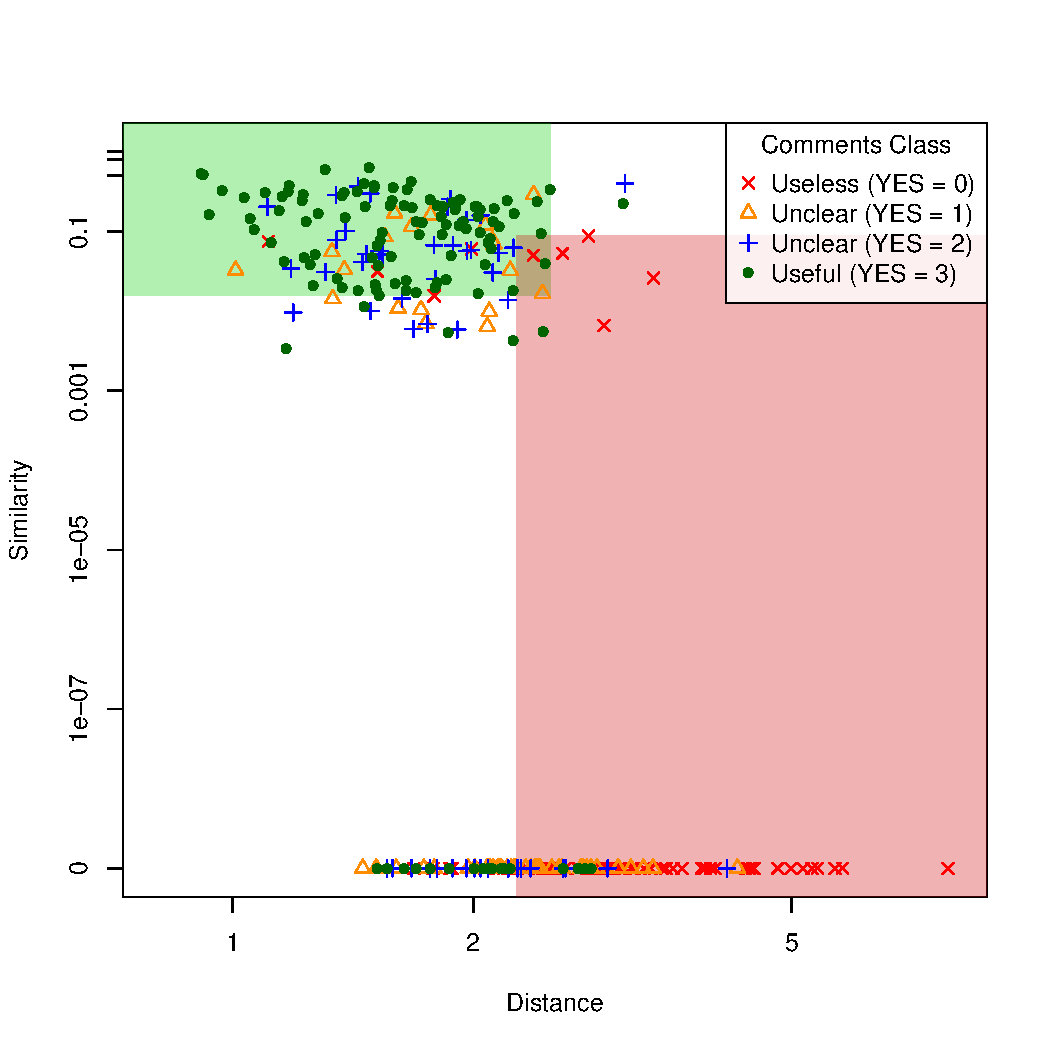
\includegraphics[scale=0.55, trim=0 0 30 50, clip=true]{scatter_log}
\caption{The similarity and distance plot of the training data.
The symbol represents the score, which ranges from 0 to 3.}
\label{fig:scatter}
\end{figure}

\noindent \textbf{RQ2: Do code reviewers intensively discuss on the proposed changes?}\\
\pick{The questions: How many \% automatic / useful/ useless/ unclear messages for each reviews? Does these numbers have a relationship with factor of code review (e.g. reviewing time)?}

\pick{If there is high \% of useless messages, it means ineffective review, isn't it?}

\noindent \textbf{RQ3: Does this approach practical and cost-effective for large-scale projects?}\\


%\subsection{Model Generation}

%% the criteria that were found
%From our training data,
%the following criteria have been obtained that maximizes the F$_1$ score:
%
%Criteria to find samples with score of 3 (``positive''):
%\begin{gather*} similarity \geq 0.015528 \text{ and } distance \leq 2.494944
%\\ \text{(F$_1$-score: 0.741313)} \end{gather*}
%
%Criteria to find samples with score of 0 (``negative''):
%\begin{gather*} similarity \leq 0.087522 \text{ and } distance \geq 2.265679
%\\ \text{(F$_1$-score: 0.725389)}\end{gather*}
%
%Note that these constant values can vary from project to project, and thus is not a universal constant.
%
%% run result
%
%Running our model against the training data gives us the result displayed in the following table.
%In the table, \emph{Neither} means that the comment did not meet either criteria, while \emph{Overlap} means that the comment  met both ``positive'' and ``negative'' criteria.
%
%\begin{center}
%\begin{tabular}{|r|rrrr|}
%\hline
%& \bfseries 0 & \bfseries 1 & \bfseries 2 & \bfseries 3 \\
%\hline
%Negative & 69 & 23 & 7 & 6 \\
%Neither & 12 & 24 & 20 & 20 \\
%Overlap & 1 & 1 & 0 & 1 \\
%Positive & 4 & 13 & 24 & 95 \\
%\hline
%\end{tabular}
%\end{center}
%
%As expected, most comments classified as \emph{negative} have score of 0 and 1,
%while most \emph{positive} comments have score of 2 and 3.
%However, some comments in every score type were classified as \emph{neither}.
%
%



% cross validation result





\section{Discussion}

% noisy data, and binary classification
Our training data is very noisy because there are disagreements between our judgment of ``usefulness.''
These samples cannot be classified as either useful or not useful.
This impacts the trade-off between the precision and recall for our model, and consequently, the F$_1$ score.

By removing the samples with scores of 1 and 2, leaving with 209 samples without disagreements, and performing 10-fold cross-validation, we received a much better average F$_1$ score of 0.896.


% tuning the F score for precision and recall
Depending on the use case, we can fine-tune the F-score to give more weight to recall or precision.
For instance, if we wanted to measure the amount of useful comments within a large dataset, we can give more weight to precision, sacrificing some good comments.
If we wanted to modify a code review software such that it displays useful comments more prominently, we can give more weight to recall.


% reasons for classification as useful or not useful
During the training process, reasons for the judgment are recorded. Examples of reasons for positive comments include:

\begin{itemize}
	\item they contain new information;
	\item they contain constructive suggestions;
	\item they discuss directly about the change; and
	\item they discuss technical matters.
\end{itemize}

Examples of reasons for negative comments include:

\begin{itemize}
	\item chatting (i.e. no new information, just communication);
	\item not discussing directly about the change;
	\item discussing about the process workflow; and
	\item discussing about Git or Gerrit itself.
\end{itemize}


% example of false positive and false negatives




\section{Threat to Validity}


\section{Conclusion and Future Work}


\IEEEpeerreviewmaketitle

\bibliographystyle{IEEEtran}

\bibliography{references}



% that's all folks
\end{document}


